% =============================================================================
% REMOVED FROM body.tex BY THE 2026-09-12 JOCS REBUILD. NOT \input BY EITHER
% BUILD. DO NOT COMPILE. This file exists so the companion paper on the
% self-auditing trust layer can be assembled without git archaeology.
%
% Provenance: every block below is copied verbatim out of docs/paper/body.tex as
% it stood at commit 47dc59d ("Amendment 2: pre-register the least-squares lower
% bound before running it"), with the original line ranges recorded above each
% block. The instruction is docs/paper/review/r2_round2.md Sec. 2.6, which found
% that ~40% of the body was trust-layer material the paper itself disclaims
% priority over, and that an editor triaging on originality reads it first.
%
% What the manuscript kept: nothing of the trust layer. sec:residual survives
% because it is an *evaluation* result -- you cannot repair a field metric with a
% physics residual -- and not because it is a system component.
%
% Labels DEFINED in the blocks below, which no longer exist in body.tex and must
% be re-declared when this material is reassembled:
%   sec:correction  prop:coverage  prop:contraction
%   sec:v2          tab:v2         tab:uq
%   sec:indist-ablation  tab:indist  fig:fig1
%   sec:ood         tab:ood        fig:fig2   fig:deepcfd  fig:cylinder
%   sec:conformal   fig:fig6       fig:fig5
%   sec:selective   fig:risk_coverage
%   sec:cost        tab:cost
%
% Labels REFERENCED by the blocks below that DO still exist in body.tex:
%   sec:method  sec:experiments  sec:interp  sec:residual  sec:limitations
%   tab:interp  tab:measure  tab:airfrans-sota
%
% Citation keys used ONLY by this material, and therefore no longer cited by the
% manuscript (they remain in refs.bib and are simply not printed by bibtex):
%   ribeiro2020deepcfd  bai2019deq  winston2020monotone  fung2022jfb
%   lakshminarayanan2017ensembles  gal2016dropout  ma2024uqno  yu2026conformalpinn
%   garg2025dfuq  jia2026multigranularity  roy2025anchor  song2026structureaware
%   gopakumar2025pre  mukherjee2026certification  beckerrannacher2001dwr
%   hillebrecht2025posteriori
% Re-check this list against the reassembled text before running bibtex.
% =============================================================================


% -----------------------------------------------------------------------------
% BLOCK 1 -- Introduction, contributions 5 and 6 of six.
% Original body.tex lines 195-210. r2_round2.md Sec. 2.6: "An editor triaging on
% originality will read the contributions list top to bottom and see three of six
% contributions that the paper itself disclaims priority over."
% -----------------------------------------------------------------------------

\item \textbf{A deployable certificate, and an honest account of what it is worth.} A
distribution-free split-conformal layer attains target coverage ($0.902{\pm}0.008$ at
$0.90$), including under distribution shift, and costs a median $1.13$\,ms against a
$3822$\,ms solve. As a detector the residual reaches AUROC $0.871$ on worst-decile field
error, but a \emph{physics-free} ensemble $\sigma$ does at least as well ($0.894$) and a
paired bootstrap cannot separate them; it is the \emph{fusion} that reaches $0.905$ and
recovers ${\approx}91\%$ of the oracle. The one place physics wins outright is the
engineering quantity, $|\Delta C_D|$ (AUROC $0.952$). The monotone-residual acceptance
gate admits a step on $99.8\%$ of deployed cases and lowers true error on $89.3\%$---but
an \emph{ungated} fixed half-step does better on accuracy alone, so what the gate buys is
the certificate, not the accuracy (\autoref{sec:conformal}, \autoref{sec:selective}).

\item \textbf{A reproducible, CPU-first open-source package} (\texttt{neuroforge-cfd})
with a frozen I/O contract, interchangeable backbones, an AirfRANS loader, the
ablation/certificate harness and the figures, so every claim runs on a laptop and every
certificate is reproducible from a committed script.


% -----------------------------------------------------------------------------
% BLOCK 2 -- Related Work, "Residual-based, data-free error signals, and
% conformal UQ." Original body.tex lines 254-272. The rebuilt manuscript keeps a
% three-sentence version covering only the residual-as-error-indicator line,
% which sec:residual still needs; the conformal-UQ half went with the layer.
% -----------------------------------------------------------------------------

\paragraph{Residual-based, data-free error signals, and conformal UQ.} Closest to our
trust-signal half is work reading the PDE residual as a reference-free error indicator:
\citet{roy2025anchor} trigger a classical solver when a residual-based estimator fires in
time-marching; \citet{song2026structureaware} align epistemic-UQ bands with localised
residual structure; \citet{gopakumar2025pre} use the residual itself as a conformal
nonconformity score, obtaining coverage in \emph{residual} space with the transfer to
solution space left open. The classical answer to the same question is that residual
magnitude becomes an error estimate only when weighted by an adjoint solution
\citep{beckerrannacher2001dwr}, and its neural analogue bounds a PINN's true error by its
residual scaled by a stability constant \citep{hillebrecht2025posteriori}; both are
conditional on the residual vanishing at the exact solution, which our monitor does not
do. \citet{mukherjee2026certification} prove the corresponding convergence statement only
under additional compactness assumptions. On the UQ side, deep ensembles
\citep{lakshminarayanan2017ensembles} and MC-dropout \citep{gal2016dropout} are standard
epistemic estimators, and conformal prediction gives distribution-free coverage for
operator learning \citep{ma2024uqno}, PINNs \citep{yu2026conformalpinn}, neural operators
\citep{garg2025dfuq} and automotive surrogates \citep{jia2026multigranularity}. We propose
no new UQ method; we calibrate on the field the user actually receives---the corrected
one---and additionally test, and reject, the residual's use as a correction objective.


% -----------------------------------------------------------------------------
% BLOCK 3 -- Method, "Trust map, conformal calibration, and the correction
% operators", in full, including both propositions.
% Original body.tex lines 420-492. This subsection existed only to define the
% quantities the cut experimental sections measured; sec:residual needs only the
% monitored operator, which stays in body.tex.
% -----------------------------------------------------------------------------

\subsection{Trust map, conformal calibration, and the correction operators}
\label{sec:correction}

\paragraph{Raw trust map.} The combined PDE-residual magnitude
$\rho_{\mathrm{res}} = \sqrt{r_c^2 + r_x^2 + r_y^2 + r_{bc}^2}$ and a per-cell predictive
uncertainty $\sigma$ are each mapped to $[0,1]$ (using an absolute physical reference
scale $s = U_\infty^2/L + U_\infty/L$ when available, else a robust 95th-percentile
normalisation with an absolute floor) and fused,
\begin{equation}
e = \mathrm{clip}\!\big(w_r\, \hat{r} + w_u\, \hat{\sigma},\; 0,\; 1\big), \qquad T = 1 - e,
\end{equation}
with $w_r=0.6$, $w_u=0.4$. Uncertainty $\sigma$ is the channel-mean standard deviation
from a deep ensemble or MC-dropout.

\paragraph{Case-level versus per-cell scope.} Our quantitative trust result is
\textbf{case-level}: the field-mean residual ranks which whole predictions to distrust
(per-case Spearman $0.611$, \autoref{sec:v2}). The \emph{per-cell} spatial rank
correlation with error \emph{within} a field is weaker---$0.22{\pm}0.06$ on the
dropout-FNO at $n{=}15$, and $0.166{\pm}0.155$ on the deployed ensemble-mean field at
$n{=}200$---but scale-dependent: patch-pooling the map to $16{\times}16$ cells roughly
doubles it ($0.323{\pm}0.232$, $+0.157$, improving $93\%$ of cases; Gaussian smoothing at
$\sigma{=}4$ cells gives $+0.135$), and the pooled patches flag top-decile-error
\emph{regions} at AUROC $0.68$--$0.72$; dynamic-pressure normalisation does not help
($+0.008$) (\texttt{results/control/percell\_localization.json}). The residual is
therefore a \emph{case-level} ranker and a \emph{moderate region-level} locator, not a
per-cell error rank; per-cell claims are left to the conformal band, which uses the
calibrated $\sigma$.

\paragraph{Split-conformal calibration.} Raw $\sigma$ is uncalibrated, so a threshold on
it carries no guarantee. On a held-out calibration set we compute per-channel
nonconformity scores $s = |\hat{y} - y| / \sigma$ and take the finite-sample-corrected
$(1-\alpha)$ quantile $q$; the band $q\cdot\sigma$ then satisfies
\autoref{prop:coverage} (cf.\ \citealp{ma2024uqno}).

\begin{proposition}[Distribution-free coverage under exchangeability]
\label{prop:coverage}
If the calibration scores and a test score are exchangeable, then the split-conformal
band $q\cdot\sigma$ satisfies $\mathbb{P}\big(|\hat{y} - y| \le q\,\sigma\big) \ge
1-\alpha$.
\end{proposition}

\paragraph{Corrector and acceptance test.} A small residual CNN predicts an additive
correction conditioned on the current field, its residual map and the geometry,
$\Delta_k = c_\phi(y_k, R(y_k), x)$. A candidate $y_{k+1} = y_k + s\,\Delta_k$ is admitted
only if it does not increase the residual norm
$N(y) = \sqrt{\overline{r_c^2 + r_x^2 + r_y^2}}$, i.e.\ $N(y_k + s\,\Delta_k) \le N(y_k) +
\varepsilon$, with $s$ halved up to four times on failure; by construction
$N(y_0) \ge \dots \ge N(y_K)$. The test is satisfiable by the identity, so a corrector that
cannot reduce the residual is simply rejected---but measured, backtracking finds an
admissible damped step on $99.8\%$ of deployed cases (\autoref{sec:selective}). The
deployed corrector is instead a Deep-Equilibrium model \citep{bai2019deq}: the correction
$\delta$ is the fixed point of $T_\theta(\delta; c) = \kappa \cdot g_\theta([\delta, c])$
with $c = [\hat{y}, r(\hat{y}), \text{geom}]$, $g_\theta$ spectrally normalised
\citep{winston2020monotone} and $\kappa < 1$, trained with Jacobian-Free
Backpropagation \citep{fung2022jfb}.

\begin{proposition}[Banach contraction of the corrector]
\label{prop:contraction}
With $g_\theta$ each-layer $1$-Lipschitz and $\kappa < 1$, $T_\theta$ is a
$\kappa$-contraction in $\delta$. By the Banach fixed-point theorem the equilibrium
$\delta^{*}$ exists, is unique, and the iteration converges geometrically,
$\|\delta_k - \delta^{*}\| \le \kappa^k \|\delta_0 - \delta^{*}\|$.
\end{proposition}

Crucially $g_\theta$ is trained on \textbf{data}---it targets the correction toward truth,
with the residual as an input \emph{feature}---rather than by minimising the residual, and
at inference $\delta^{*}$ is applied directly, \textbf{without} the acceptance test. Two
scopes must be kept distinct: the DEQ contraction is in the \emph{correction variable}
$\delta$, whereas the \emph{PDE residual of the output field} is a different quantity that
can rise even as $\delta$ converges and the field error falls. After the loop, a
trust-gated \texttt{ClassicalFallback} would hand low-trust regions to an external solver;
in the present release it is an \textbf{interface with a \texttt{stub} backend} that
reports what would run without invoking one, and it bears on no quantitative claim.


% -----------------------------------------------------------------------------
% BLOCK 4 -- sec:v2, the trust-layer and corrector half. Original body.tex lines
% 1138-1190 (heading, tab:v2, "Learned correction works on a strong backbone")
% and 1242-1322 (W1 control, backbone-robust trust signal, conformal coverage,
% tab:uq). The manuscript KEPT the two force-integrator paragraphs from this
% subsection (original lines 1191-1240), which now stand as sec:forces, because
% they are a representation result about the scoring raster and not a trust
% claim.
% -----------------------------------------------------------------------------

\subsection{Backbone-agnostic trust and learned correction on a SOTA backbone}
\label{sec:v2}

We re-run the trust layer and the DEQ corrector on a \textbf{SOTA Transolver backbone}
($7.35$M parameters, 80 epochs, AirfRANS \texttt{full}, 5 seeds; corrector trained $20$
epochs with the backbone frozen), the strongest model in our study. Protocol and scoring
are identical to \autoref{sec:indist-ablation}; the sources are
\texttt{results/v2/v2\_results.json} (original 3-seed study) and
\texttt{results/control/w1\_capture.json} (identical recipe, extended to five seeds; the
extension reproduces the 3-seed corrector deltas and $\rho_{C_l}$ within pre-registered
tolerances).

\begin{table}[t]
\centering
\small
\caption{SOTA Transolver backbone ($7.35$M params, 80 ep, AirfRANS \texttt{full}), alone
vs.\ with the DEQ correction loop. 5 seeds, mean $\pm$ std (population std,
\texttt{ddof=0}). Lower MSE is better;
$\rho$ closer to 1 is better;
resid$\leftrightarrow$err $\rho > 0$ supports the trust signal. The $C_l$/$C_d$ columns
are relative error against the ground-truth field's own integrated forces, not against the
official labels; the paragraph after next states what that integrator can and cannot see.
Source: \texttt{results/control/w1\_capture.json} (5-seed extension of
\texttt{results/v2/v2\_results.json}).}
\label{tab:v2}
\resizebox{\textwidth}{!}{%
\begin{tabular}{l r r r r r r}
\toprule
metric & $\texttt{mse\_u}$ & $\texttt{mse\_v}$ & $\texttt{mse\_p}$ & $C_l$ rel.\ err & $C_d$ rel.\ err & resid$\leftrightarrow$err $\rho$ \\
\midrule
backbone & $0.133{\pm}0.017$ & $0.096{\pm}0.006$ & $644{\pm}63$ & $5.7\%$ & $7.6\%$ & $0.611{\pm}0.054$ \\
\ + DEQ loop & $0.122{\pm}0.015$ & $0.076{\pm}0.006$ & $485{\pm}39$ & $5.5\%$ & $6.8\%$ & $0.612{\pm}0.046$ \\
$\Delta$ & $-8\%$ & $-21\%$ & $-25\%$ & $-0.2$pp & $-0.8$pp & $+0.002$ \\
\bottomrule
\end{tabular}%
}
\end{table}

\paragraph{Learned correction works on a strong backbone.} The DEQ corrector reduces
volume field MSE on \textbf{all five seeds}: $\texttt{mse\_u}$ $-8\%$, $\texttt{mse\_v}$
$-21\%$, $\texttt{mse\_p}$ $-25\%$. \textbf{Surface-pressure} MSE is the one channel it
does \emph{not} improve: essentially flat at $9843\rightarrow9899$ ($+0.6\%$; per-seed
$-1/-1/+2/+2/+1\%$). Internal force-ranking consistency is held at $\rho_{C_l}=0.999$ and
$\rho_{C_d}=0.996$. These deltas are within-backbone---the same architecture against
itself, on one measure---so they are untouched by \autoref{tab:measure}. What
\autoref{tab:measure} does touch is the cross-method reading: area-uniform, the corrected
$\texttt{mse\_p}=485$ is $6.5\times$ the $75.0$ a parameter interpolator reaches with no
learning, while node-weighted the ordering is the other way round. Under either weighting
the $-25\%$ is a relative improvement to a learned backbone and not a field-accuracy
record; its value lies in the channels where interpolation fails---$u$, $\nu_t$ and the
first cell off the wall---and in being reference-free at deployment, which an interpolator
carrying $210$\,MB of training fields is not.

\paragraph{The gain comes from the learned correction, not from feeding it the residual
(W1 control).} To isolate \emph{why} the corrector helps, we train the same DEQ corrector
two ways under identical architecture, data, optimiser, schedule and seeds, differing only
in whether the 3 residual input channels carry the real residual (WITH) or are permanently
zeroed at both train and inference (NULL). Across 5 seeds the null corrector
\textbf{matches or slightly exceeds} the deployed one: the per-seed paired difference is
negative on all 5 seeds for both $\texttt{mse\_u}$ and $\texttt{mse\_speed}$ (mean
$\approx -0.005$ on a $\approx 0.12$ base, $\approx 4\%$; WITH beats NULL on $0/5$ seeds;
\texttt{results/control/w1\_capture.json}). The improvement is attributable to the learned
correction architecture, not to residual-conditioning---consistent with the residual's role
elsewhere: it tells you \emph{which} predictions are wrong, not \emph{how} to fix them. The
deployed system keeps the residual input because it is already computed for the trust
layer, so conditioning on it costs nothing extra. One caveat qualifies the null
(\autoref{sec:method}): those input channels are built from the wider differentiable
stencil, whose larger kernel we have not excluded as an explanation.

\paragraph{The trust signal is backbone-robust.} On this SOTA backbone the bare
residual--error correlation is already strong ($0.611{\pm}0.054$ over five
seeds---per-seed $0.611/0.652/0.613/0.667/0.511$, positive on every seed), against
$\approx 0.40$ for the bare weak backbone (\autoref{tab:indist}); the corrector barely
moves it ($0.612{\pm}0.046$). We add a third, architecturally distinct data point: a
message-passing GNN (MeshGraphNet, param-matched at $7.35$M, 3 seeds, bare backbone),
where the bare case-level residual--error Spearman is $0.851{\pm}0.058$
(\texttt{results/mgn/mgn\_results.json}). Across a spectral grid Geo-FNO, an
attention/point-cloud Transolver and a message-passing GNN the correlation is consistently
\emph{positive}, though variable in strength. \textbf{The MeshGraphNet arm is not a
like-for-like third point}: that model was trained on $16$k-point subsamples and evaluated
at the full $\approx180$k points, and our own density control
(\texttt{results/control/mgn\_density\_control.json}) returns \textsc{density-driven} with
an MSE ratio of $2.44$. The control measures MSE on four cases and carries no rank
correlation, so it does not establish that $0.851$ is \emph{itself} a density artifact---but
the $0.40$--$0.85$ range should be read as $0.40$--$0.61$ among the arms trained and
evaluated at matched density. The detector remains positive on all three.

\paragraph{Coverage holds under both uncertainty estimators; only an ensemble is
adaptive.} Split-conformal calibration of the pressure channel at $\alpha=0.1$ attains
target coverage with \emph{either} estimator: $0.902{\pm}0.008$ with MC-dropout (3 seeds)
and $0.915$ with a deep ensemble (single run), both at the $0.90$ target. Coverage was
never the difficulty---\textbf{adaptivity} was. With MC-dropout this near-deterministic
model has near-degenerate $\sigma$ at dropout $0.05$, so coverage is delivered by a
\textbf{near-constant} band: the conformal quantile is enormous ($\approx 1.5$--$1.7\times
10^{9}$) and the reliability ECE is $\approx 0.31$. Replacing it with a deep ensemble of
$M{=}5$ independently trained Transolvers---per-cell standard deviation across members as
$\sigma$---converts that into a genuinely input-adaptive band while preserving coverage
(\autoref{tab:uq}): on the same $100/100$ split the quantile drops to $q=2.35$, ECE
improves to $\mathbf{0.074}$, and coverage holds at $0.915$ (consistent with the
$\approx{\pm}0.03$ binomial spread at $n_{\text{test}}=100$). This is a single ensemble
training run; the calibration/test \emph{split} is not the fragile part---re-drawing it
$20$ times leaves coverage at $0.899{\pm}0.009$ with $q=2.26{\pm}0.05$ on pressure
(\autoref{sec:conformal}). The ensemble mean is also more accurate than any single member
($\rho_{C_l}=0.9995$, $\rho_{C_d}=0.998$, $C_l/C_d$ relative force error $4.4\%/5.7\%$)
and more accurate than the DEQ-corrected single backbone
($\texttt{mse\_u/v/p}=0.077/0.058/440$ against $0.116/0.079/471$), so we do not claim the
corrector is the best available accuracy mechanism. The two answer different questions on
a cost axis: the ensemble is the better \emph{accuracy} play when $5\times$ the training is
affordable, the corrector the better \emph{cheap} play; an $M$-subset study shows $M{=}2$
already supports the triage decisions while full band adaptivity needs $M{\approx}4$--$5$
(\autoref{sec:limitations}).

\begin{table}[t]
\centering
\small
\caption{Conformal calibration of the pressure channel on the SOTA Transolver backbone
($\alpha=0.1$, $100/100$ cal/test split): MC-dropout vs.\ a deep ensemble ($M{=}5$). Both
attain target coverage; only the deep ensemble yields an input-adaptive band (finite $q$,
low ECE). MC-dropout: 3 seeds (mean$\pm$std); deep ensemble: single ensemble training
(split-to-split spread over 20 calibration/test re-draws: coverage $0.899{\pm}0.009$,
$q=2.26{\pm}0.05$; \autoref{sec:conformal}). Sources:
\texttt{results/v2/v2\_results.json}, \texttt{results/uq\_ensemble/uq\_results.json}.}
\label{tab:uq}
\begin{adjustbox}{max width=\textwidth}
\begin{tabular}{l c c c l}
\toprule
$\sigma$ estimator & coverage (target $0.90$) & $q$ & ECE ($\downarrow$) & band \\
\midrule
MC-dropout ($p{=}0.05$) & $0.902{\pm}0.008$ & $\approx 1.6\times 10^{9}$ & $\approx 0.31$ & near-constant \\
deep ensemble ($M{=}5$) & $0.915$ & $2.35$ & $\mathbf{0.074}$ & \textbf{adaptive} \\
\bottomrule
\end{tabular}
\end{adjustbox}
\end{table}


% -----------------------------------------------------------------------------
% BLOCK 5 -- sec:indist-ablation, the weak grid backbone, in full.
% Original body.tex lines 1324-1388, including tab:indist and fig:fig1.
% The grid backbone leaves the manuscript entirely with this block: its two rows
% in tab:interp and its row in tab:interp_std were deleted with it, as was
% fig:fig3 in the appendix, which plotted its gap to Transolver.
% -----------------------------------------------------------------------------

\subsection{The grid backbone: the corrector trades accuracy for trust signal}
\label{sec:indist-ablation}

\begin{table}[t]
\centering
\small
\caption{In-distribution AirfRANS \texttt{full} ablation, 3 seeds, mean $\pm$ std
(population std). Lower MSE is better; $\rho$ closer to 1 is better; resid$\leftrightarrow$err
$\rho > 0$ supports the trust signal. Bold marks the best arm per column among the
physics-loss arms; the physics-loss-free arm (starred where best overall) is reported
separately because it removes the physics objective entirely. See \autoref{fig:fig1}.}
\label{tab:indist}
\resizebox{\textwidth}{!}{%
\begin{tabular}{l r r r r r r r}
\toprule
arm & $\texttt{mse\_u}$ & $\texttt{mse\_v}$ & $\texttt{mse\_p}$ & surf.\ $\texttt{mse\_p}$ & $\rho_{C_l}$ & $\rho_{C_d}$ & resid$\leftrightarrow$err $\rho$ \\
\midrule
backbone & $3.479{\pm}0.105$ & $\mathbf{0.385{\pm}0.012}$ & $\mathbf{2444.8{\pm}120.7}$ & $548823{\pm}27946$ & $0.9868{\pm}0.0005$ & $0.895{\pm}0.013$ & $0.397{\pm}0.003$ \\
backbone (no phys.\ loss) & $\mathbf{1.995{\pm}0.042}$ & $0.323{\pm}0.008^{*}$ & $1963.5{\pm}55.5^{*}$ & $1123649{\pm}104822$ & $\mathbf{0.9920{\pm}0.0002}$ & $\mathbf{0.945{\pm}0.008}$ & $0.605{\pm}0.016$ \\
backbone + local corr. & $3.482{\pm}0.058$ & $0.398{\pm}0.007$ & $2469.4{\pm}71.0$ & $541534{\pm}20453$ & $0.9854{\pm}0.0017$ & $0.888{\pm}0.012$ & $0.389{\pm}0.031$ \\
backbone + DEQ corr. & $3.457{\pm}0.811$ & $0.880{\pm}0.064$ & $3832.7{\pm}331.3$ & $\mathbf{361681{\pm}12273}$ & $0.9856{\pm}0.0017$ & $0.923{\pm}0.014$ & $\mathbf{0.827{\pm}0.002}$ \\
\bottomrule
\end{tabular}%
}
\end{table}

This ablation uses the \textbf{weak grid backbone}; it establishes the backbone-dependence
we report as a finding, and should be read against \autoref{sec:v2}, where the same
corrector \emph{does} reduce field MSE. Here the DEQ corrector is \textbf{flat} on volume
$\texttt{mse\_u}$ ($3.457$ vs $3.479$; per-seed deltas sign-inconsistent, 2/3, so noise)
and \textbf{worse} on $\texttt{mse\_v}$ ($+129\%$, 3/3, non-overlapping distributions) and
$\texttt{mse\_p}$ ($+57\%$, 3/3); the feed-forward \texttt{local} corrector helps on
\textbf{nothing}. The DEQ arm buys surface-pressure MSE ($-34\%$, 3/3) and a slightly
better drag ranking ($0.895\rightarrow0.923$, 3/3) at a measured cost to volume velocity
and pressure. We do \textbf{not} claim the corrector improves accuracy in aggregate on
this backbone.

\paragraph{The detector succeeds, and a control sharpens the thesis.} The same DEQ arm
roughly \textbf{doubles} the residual--error Spearman correlation,
\textbf{$0.397\rightarrow0.827$} (3/3, std $\approx 0.002$, Cohen's $d \approx 175$;
effect sizes use the population std, matching the tables)---the largest, cleanest effect
in the table. Separately, removing the physics loss entirely \textbf{improves}
$\texttt{mse\_u}$, $\texttt{mse\_v}$, $\texttt{mse\_p}$, $\rho_{C_l}$, $\rho_{C_d}$ and
the residual--error correlation (all 3/3), at the cost of \textbf{doubling}
surface-pressure MSE ($549\text{k}\rightarrow1124\text{k}$, 3/3). The physics-loss-free
backbone is in fact the \textbf{best force-ranking model in the table} ($\rho_{C_d}$
$0.945$, $\rho_{C_l}$ $0.992$)---better than any corrected model, with no correction loop
at all---so we explicitly do \textbf{not} claim the loop delivers best-in-class force
ranking. The physics objective buys surface-pressure fidelity and a strong trust signal,
not volume accuracy or force ranking on this weak backbone.

\begin{figure}[t]
\centering
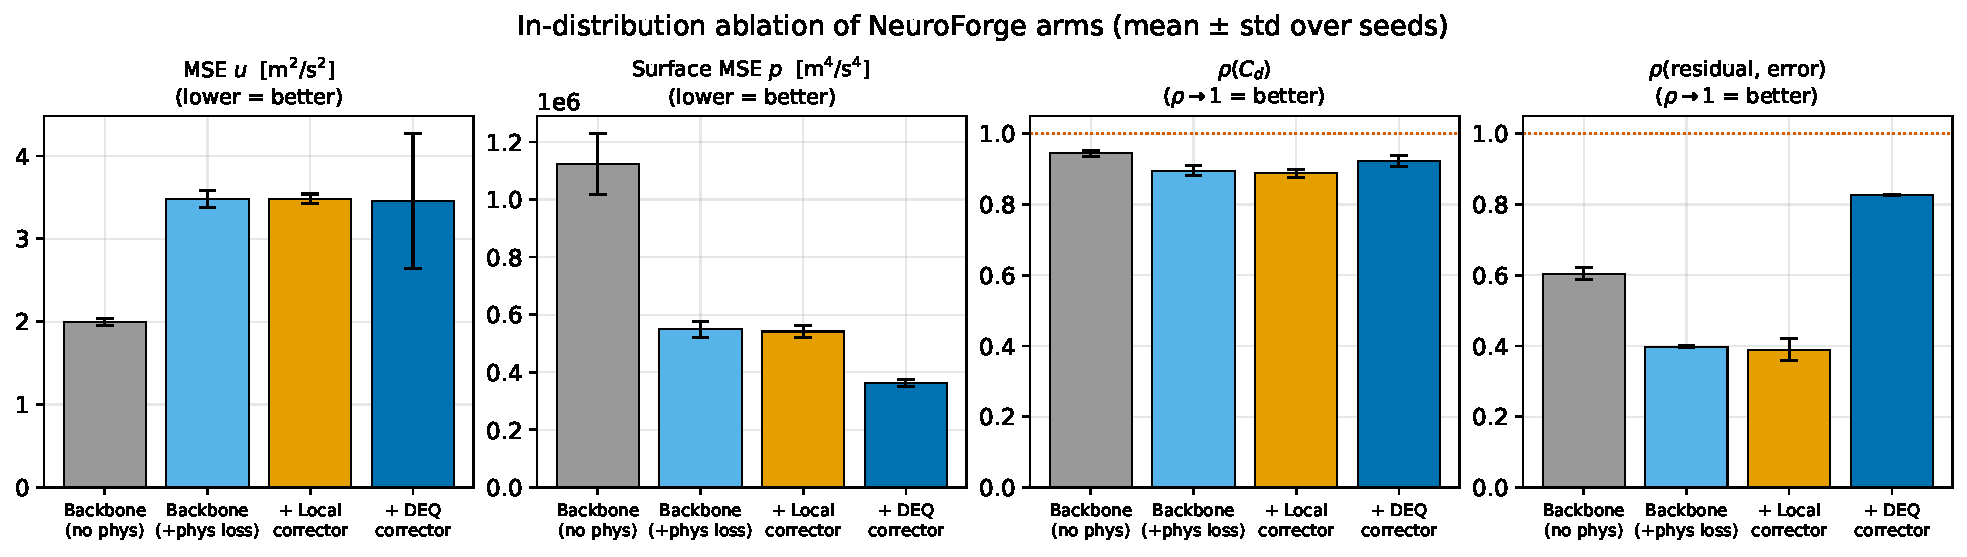
\includegraphics[width=0.85\textwidth]{../../results/figures/fig1_ablation_indist.pdf}
\caption{In-distribution ablation (\autoref{tab:indist}): the DEQ corrector lifts the
trust signal ($0.40\rightarrow0.83$) and surface fidelity while regressing volume
$\texttt{mse\_v}$/$\texttt{mse\_p}$.}
\label{fig:fig1}
\end{figure}

\paragraph{Version note for readers of the preprint.} The single-seed figures reported in
earlier public versions---$\rho_{C_l}$ rising $0.924\rightarrow0.958$ and surface MSE
$-25\%$ under the corrector---do not replicate: across 3 seeds the backbone already sits
at $\rho_{C_l}=0.987$ and the DEQ corrector at $0.986$, flat-to-slightly-worse and
sign-inconsistent. \autoref{tab:indist} supersedes them.


% -----------------------------------------------------------------------------
% BLOCK 6 -- sec:ood, in full. Original body.tex lines 1390-1484, including
% tab:ood, fig:fig2, the DeepCFD second-dataset paragraph, fig:deepcfd, and the
% cylinder cross-geometry paragraph. fig:cylinder itself lived in the appendix
% and is preserved as BLOCK 10 below.
% -----------------------------------------------------------------------------

\subsection{Residuals detect under distribution shift}
\label{sec:ood}

We evaluate each arm on the regime-disjoint \texttt{reynolds} and \texttt{aoa} splits
(trained on the train range, tested on the held-out range---true extrapolation);
\autoref{tab:ood} reports both.

\begin{table}[t]
\centering
\small
\caption{Out-of-distribution AirfRANS ablation (regime-disjoint train$\rightarrow$test),
3 seeds, mean $\pm$ std. The full four-arm table is in
\texttt{results/full\_research/ood/ablation\_ood.md}. See \autoref{fig:fig2}.}
\label{tab:ood}
\resizebox{\textwidth}{!}{%
\begin{tabular}{l l r r r r r r r}
\toprule
task & arm & $\texttt{mse\_u}$ & $\texttt{mse\_v}$ & $\texttt{mse\_p}$ & surf.\ $\texttt{mse\_p}$ & $\rho_{C_l}$ & $\rho_{C_d}$ & resid$\leftrightarrow$err $\rho$ \\
\midrule
reynolds & backbone & $16.218{\pm}0.746$ & $1.187{\pm}0.149$ & $7220.7{\pm}612.2$ & $964641{\pm}61419$ & $0.950{\pm}0.008$ & $0.893{\pm}0.009$ & $0.748{\pm}0.077$ \\
reynolds & + DEQ & $5.300{\pm}1.544$ & $1.208{\pm}0.255$ & $6469.5{\pm}438.0$ & $652281{\pm}45390$ & $0.943{\pm}0.008$ & $0.915{\pm}0.009$ & $0.742{\pm}0.041$ \\
aoa & backbone & $4.312{\pm}0.077$ & $1.310{\pm}0.039$ & $6042.8{\pm}242.5$ & $2000592{\pm}55092$ & $0.963{\pm}0.003$ & $0.926{\pm}0.002$ & $0.314{\pm}0.064$ \\
aoa & + DEQ & $3.538{\pm}0.681$ & $1.407{\pm}0.089$ & $4620.6{\pm}170.2$ & $1042711{\pm}78298$ & $0.966{\pm}0.006$ & $0.905{\pm}0.013$ & $0.746{\pm}0.027$ \\
\bottomrule
\end{tabular}%
}
\end{table}

\paragraph{The trust signal is regime-invariant.} On the \texttt{aoa} split the bare
backbone's residual--error correlation \textbf{collapses to $0.314$}, while the
DEQ-corrected model holds it at \textbf{$0.746$} (3/3, Cohen's $d \approx 8.9$,
non-overlapping: every corrected seed $\ge 0.72$, every backbone seed $\le 0.38$). On
\texttt{reynolds} both are high ($\approx 0.74$--$0.75$). The residual is a reliable
detector exactly where detection matters most. The same ablation shows the DEQ corrector
reducing the in-distribution$\rightarrow$OOD \emph{gap} on volume velocity, volume
pressure and surface pressure (e.g.\ \texttt{reynolds} $\texttt{mse\_u}$
$16.2\rightarrow5.3$, \texttt{aoa} surf.\ $\texttt{mse\_p}$
$2.00\text{M}\rightarrow1.04\text{M}$, both 3/3), which we report as an observation about
the loop's behaviour and \textbf{not} as a generalisation guarantee, preserving two
negatives. (i)~\textbf{$\texttt{mse\_v}$ is an attenuated-regression artifact, not a
gain}: the corrector's \emph{absolute} OOD $\texttt{mse\_v}$ is worse than the backbone in
every regime ($0.880/1.208/1.407$ vs $0.385/1.187/1.310$); its gap only looks smaller
because its in-distribution value is already inflated. (ii)~\textbf{Drag ranking is
task-dependent}: $\rho_{C_d}$ improves on \texttt{reynolds} ($0.893\rightarrow0.915$, 3/3)
but \textbf{regresses on \texttt{aoa}} ($0.926\rightarrow0.905$, worse on all 3 seeds).
Methodological caveat: the in-distribution reference is the \texttt{full} split, so the
gap mixes a train-set change with regime shift, and the \texttt{aoa} $\texttt{mse\_u}$
effect, while 3/3 directional, is seed-0-dominated.

\begin{figure}[t]
\centering
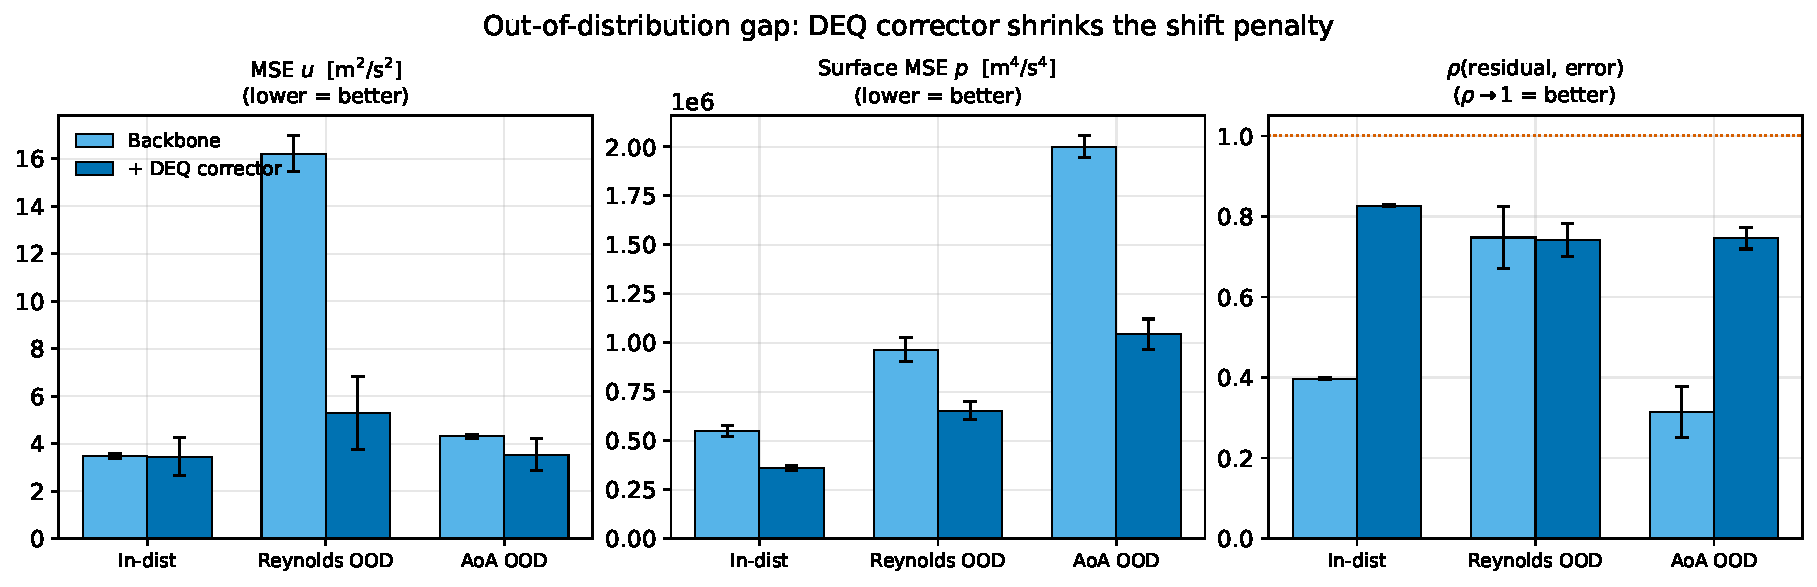
\includegraphics[width=0.85\textwidth]{../../results/figures/fig2_ood_gap.pdf}
\caption{OOD gap and the regime-invariant trust signal (\texttt{aoa}
$0.31\rightarrow0.75$); the bare backbone's signal collapses, the corrected model's holds.}
\label{fig:fig2}
\end{figure}

\paragraph{A second dataset: the trust signal generalises beyond AirfRANS.} We evaluate
the residual trust signal on \textbf{DeepCFD} \citep{ribeiro2020deepcfd}---2-D laminar
incompressible flow over bluff bodies: a different geometry family \emph{and} a different
regime. We train an FNO backbone (3 seeds) on an out-of-distribution split holding out the
largest bodies and measure the same per-case residual--error Spearman correlation
(\texttt{results/deepcfd/deepcfd\_results.json}). The trust signal holds
(\autoref{fig:deepcfd}): \textbf{$0.770 \pm 0.119$}, comparable to---indeed above---the
AirfRANS Transolver value ($0.611$). The error spread is genuine (per-case rel-$L_2$
median $0.063$, max $0.136$), and per-seed case-level bootstrap $95\%$ CIs ($10^4$
resamples) are $[0.65,0.77]$, $[0.58,0.72]$ and $[0.91,0.95]$, all far from zero
(\texttt{results/control/bootstrap\_spearman\_ci.json}). A mechanistic reason it can be
\emph{sharper} than the turbulent case: laminar flow has $\nu_t=0$, so the residual is the
\emph{exact} Navier--Stokes residual with no closure ambiguity.

\begin{figure}[t]
\centering
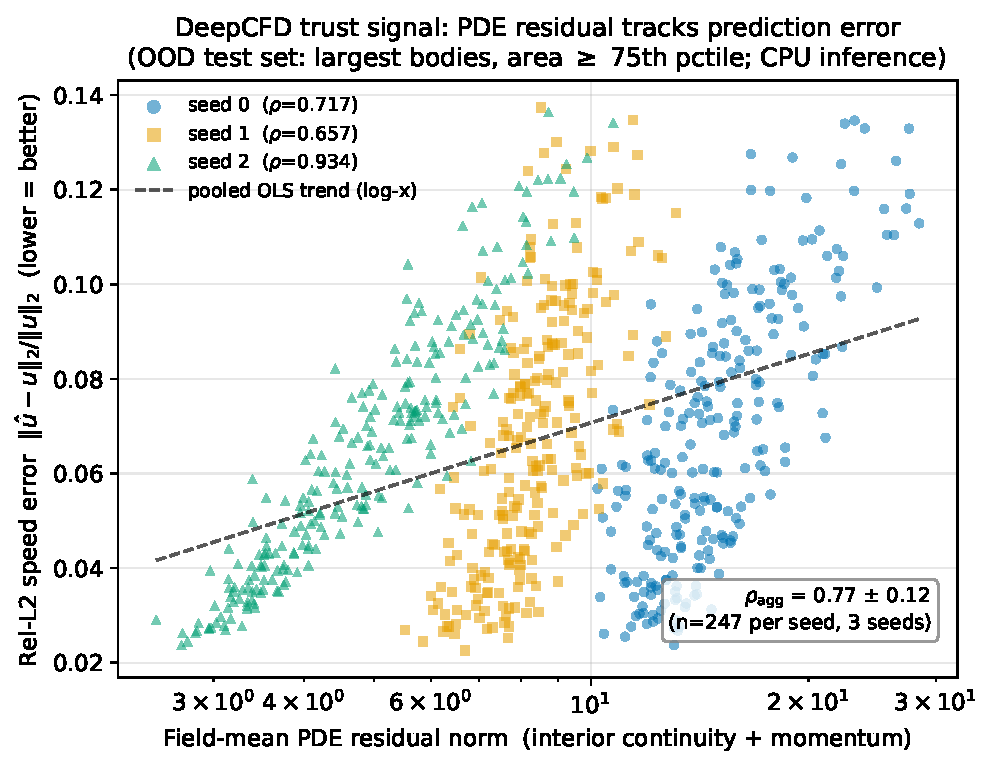
\includegraphics[width=0.75\textwidth]{../../results/figures/fig_deepcfd_trust.pdf}
\caption{The trust signal generalises to a second dataset (DeepCFD, 2-D laminar flow over
bluff bodies; OOD held-out-largest-body split, 3 seeds). Per-case field-mean PDE residual
norm vs.\ rel-$L_2$ speed error: a low residual tracks a low error, as on AirfRANS.
Per-case Spearman $\rho=0.77{\pm}0.12$ (per seed $0.72/0.66/0.93$; the trend holds
\emph{within} each seed).}
\label{fig:deepcfd}
\end{figure}

\paragraph{A geometry the model never saw (qualitative).} We run the airfoil-trained
Transolver on a \emph{cylinder} and ask not whether the prediction is good (it is not) but
whether the residual registers the geometry as out-of-distribution. It does, in the
residual \emph{magnitude}: normalising each case's residual by its freestream $U^2$, the
dimensionless far-field residual is $\approx 7\times$ higher on the cylinder (median
$\approx 30\times$; \autoref{fig:cylinder}). The gap holds in the \emph{far field}, away
from any wall, so it is a genuine geometry-OOD effect rather than a near-wall
discretisation or velocity-scale artifact. We report a control that \emph{refutes} the
tempting spatial reading: the residual's bright near-body ring is a generic no-slip-wall
feature, not an OOD localiser---in-distribution airfoils with good predictions show the
same near-body-vs-far-field concentration ratio ($\approx 23$) as the cylinder ($\approx
18$). The out-of-distribution signal is the field-wide residual \emph{magnitude}, not its
spatial ratio.


% -----------------------------------------------------------------------------
% BLOCK 7 -- sec:conformal, in full. Original body.tex lines 1486-1579,
% including fig:fig6 and fig:fig5.
% -----------------------------------------------------------------------------

\subsection{The conformal trust layer: coverage, contraction, and what the floor costs}
\label{sec:conformal}

\paragraph{Contraction.} Iterating the learned DEQ operator from a random initialisation
on 24 real AirfRANS cases, the measured per-step ratio
$\|\delta_{k+1}-\delta^{*}\|/\|\delta_k-\delta^{*}\|$ (in the geometric regime, before the
$\sim 10^{-7}$ solve floor) has \textbf{median 0.78} and maximum $0.86$---strictly below
the design bound $\kappa = 0.9$ of \autoref{prop:contraction}---and reaches a relative
distance of $10^{-5}$ to the
fixed point in a median of 37 steps
(\texttt{results/certificates/h5\_contraction.json}). The corrector contracts as designed;
this is a property of the \emph{operator}, separate from whether minimising the output's
PDE residual helps the field (it does not, \autoref{sec:residual}).

\paragraph{In-distribution coverage.} With per-cell MC-dropout $\sigma$ (16 passes) and a
100/100 calibration/test split, split-conformal calibration at $\alpha = 0.1$ attains
per-channel coverage of \textbf{0.911 ($u$), 0.928 ($v$), 0.942 ($p$)}---all in the
$[0.85, 0.95]$ band and conservatively above the $0.90$ target, as the $\ge 1-\alpha$
guarantee requires. The conformal multipliers ($q = 0.77, 1.30, 1.75$) both tighten an
over-dispersed and widen an under-dispersed raw $\sigma$, so the calibration is doing real
work, and coverage tracks $1-\alpha$ across a sweep of $\alpha$ (\autoref{fig:fig6}). The
reliability diagram is exact at the target level but over-covers at lower nominal levels
(ECE $u/v/p = 0.064/0.093/0.130$), the signature of a heavy-tailed $|\text{error}|/\sigma$
ratio; we therefore claim coverage at the chosen $\alpha$, \textbf{not} full
distributional calibration.

\paragraph{The certificate is calibrated on the deployed, corrected field.}
Split-conformal calibration applies to whatever predictor it scores, and a raw-backbone
certificate does \textbf{not} transfer unchanged through a corrector. A within-run
frozen-$q$ contrast on the dropout-FNO---same $q$, same input-conditional $\sigma$, same
cases, only the raw vs.\ corrected error map ($15/15$ split)---shows the direction of the
coverage change tracking the direction of the error change: where the corrector enlarges
the error the raw band drops below target ($v$ $0.896\rightarrow0.819$, $p$
$0.864\rightarrow0.777$), and where it shrinks the error the band over-covers ($u$
$0.856\rightarrow0.888$). Re-fitting $q$ on the corrected calibration field restores
coverage ($v$ $0.819\rightarrow0.894$, $p$ $0.777\rightarrow0.834$) and sharpens it where
it was loose ($u$ $0.888\rightarrow0.874$). These estimates are directional at $n=15$
($\approx\pm0.05$ standard error) but reproduce on an independent $20/20$ split. On the
deployed Transolver we verify it \emph{directly}: with $\sigma$ the frozen five-member
ensemble std and the scored field replaced by the DEQ-corrected output, at the production
$100/100$ split and across all three corrector seeds
(\texttt{results/uq\_ensemble/w2\_conformal\_corrected.json}; a faithfulness gate
reproduces the published backbone certificate, $q{=}2.35$, coverage $0.915$, exactly),
re-fitting $q$ gives a valid certificate (coverage $u/v/p = 0.88/0.91/0.91$ against the
$0.90$ target), and because the corrected field's error is lower at frozen $\sigma$ that
accuracy propagates into proportionally tighter intervals ($q$: $v$
$2.58\rightarrow2.34$, $p$ $2.35\rightarrow2.10$ on every seed). Applying the
\emph{backbone's} own $q$ to the corrected field over-covers on $v$ and $p$ ($\approx
0.93$) while $u$ holds at $\approx 0.88$, inherited from the backbone's own heavy-tailed
$u$ band ($0.881$) rather than introduced by the corrector. Re-drawing the split $20$
times (\texttt{results/uq\_ensemble/multisplit\_conformal.json}) leaves coverage tightly
centred on target in \emph{every} arm and channel ($0.895$--$0.902$, split-to-split std
$\le 0.014$); the corrected-field sharpening is robust, with pressure $q$ dropping from
$2.26 \pm 0.05$ to $2.02$--$2.07$ and $v$ from $2.55 \pm 0.05$ to $2.28$--$2.31$, while
the heavy-tailed $u$ channel is mixed.

\begin{figure}[t]
\centering
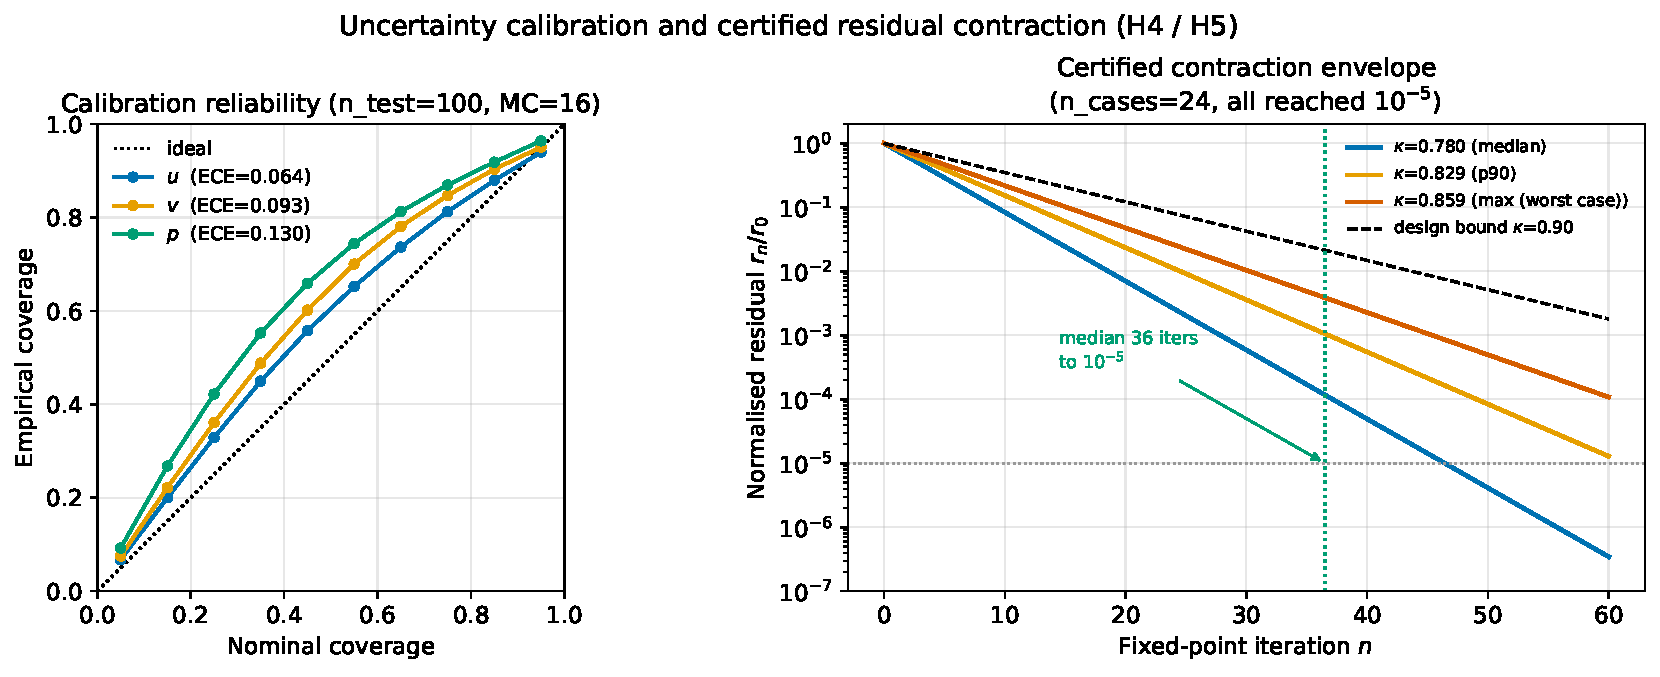
\includegraphics[width=0.85\textwidth]{../../results/figures/fig6_reliability_contraction.pdf}
\caption{In-distribution reliability / coverage-vs-$\alpha$ and the measured DEQ
contraction ($0.78 < 1$).}
\label{fig:fig6}
\end{figure}

\paragraph{Out-of-distribution coverage (empirical, not a guarantee).} Calibrating $q$ on
the in-distribution \texttt{full} split and evaluating on the OOD splits, coverage stays
in the target band: $u$ $0.90/0.91/0.91$, $v$ $0.91/0.94/0.92$, $p$ $0.92/0.94/0.90$
(full / reynolds / aoa) (\autoref{fig:fig5}). \textbf{This is an empirical observation,
not a guarantee.} The conformal guarantee assumes exchangeable calibration and test draws,
which fails under shift; coverage nonetheless holds because the MC-dropout $\sigma$
inflates appropriately on shifted inputs, so the same $q$ still brackets the larger errors.

\begin{figure}[t]
\centering
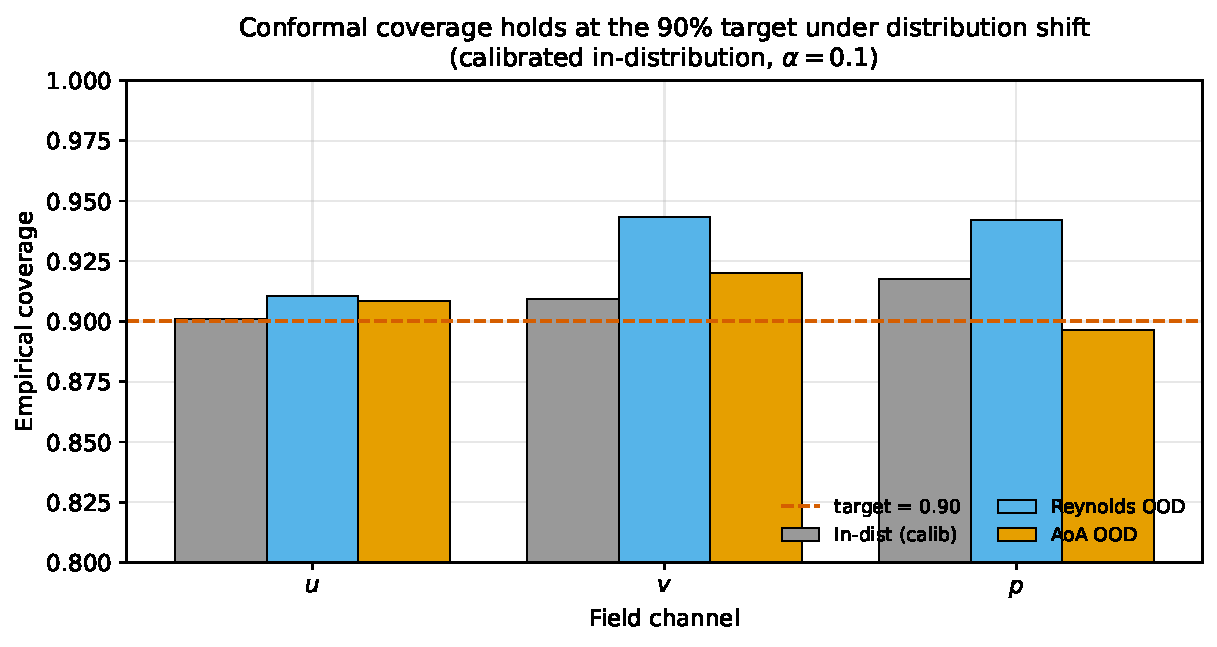
\includegraphics[width=0.85\textwidth]{../../results/figures/fig5_ood_coverage.pdf}
\caption{Conformal coverage stays in-band on OOD splits (empirical, via $\sigma$
inflation).}
\label{fig:fig5}
\end{figure}

\paragraph{What the floor costs the certificate: valid, but wide.} The quantity an
engineer actually wants bounded is a force coefficient. Conformalising the monitored
residual against $|\Delta C_D|$ over $400$ random half-splits at a $0.90$ target on the
deployed backbone gives coverage $0.901$--$0.903$ across three seeds---so the guarantee
holds, and the floor does \emph{not} invalidate split conformal, which needs only
exchangeability. What the floor destroys is tightness: the median bound is
$\mathbf{6.5}$--$\mathbf{7.9\times}$ the median drag error it certifies. We tested the
obvious explanation---that the floor is what makes it wide---and it is \emph{wrong}:
removing the floor exactly, by scoring $\|R_h(\hat u)-R_h(u^\star)\|$, makes the bound
\textbf{wider} ($7.35\times$ to $11.33\times$, $3/3$ seeds; a scale-invariance gate passes
at exactly $0.0$). What sets the width is the heavy tail of the drag error itself: its
$0.9$ quantile is $15.1\times$ its median, so an uninformative score would give
$15.1\times$. Against that reference the monitor is worth $\mathbf{2.34\times}$, and that
is the honest statement of what it buys.


% -----------------------------------------------------------------------------
% BLOCK 8 -- sec:selective, in full. Original body.tex lines 1581-1654,
% including fig:risk_coverage.
% -----------------------------------------------------------------------------

\subsection{From correlation to decisions, and where the physics earns its place}
\label{sec:selective}

A rank correlation of $0.6$ can sound modest, so we measure what the trust signal is
\emph{for}: deciding which predictions to reject
(\texttt{results/selective/selective\_prediction.json}; \autoref{fig:risk_coverage}). On
the $200$ AirfRANS test cases (ensemble-mean arm) the residual detects worst-decile-error
cases with AUROC $0.871$; the ensemble $\sigma$ alone gives $0.894$; the rank-fused score
reaches \textbf{AUROC $0.905$} (AUPRC $0.681$ against a $0.10$ prevalence baseline). The
same residual score transfers: AUROC $0.89$--$0.91$ on the three DEQ-corrected arms and
$0.83$--$0.98$ on the three DeepCFD OOD seeds. In risk--coverage terms, rejecting the
$10\%$ least-trusted cases by the fused score reduces the retained mean relative-$L_2$
error from $0.0040$ to $0.0035$---recovering $\approx 91\%$ of the error reduction an
\emph{oracle} rejecting by true error could achieve at that budget (the residual alone
recovers $\approx 67\%$; random rejection recovers none). Case-level bootstrap $95\%$ CIs
($10^4$ resamples) put the ensemble-arm residual correlation at $0.610$ $[0.506, 0.698]$
and the fused score at $0.703$ $[0.615, 0.773]$; every arm's CI excludes zero by a wide
margin.

\begin{figure}[t]
\centering
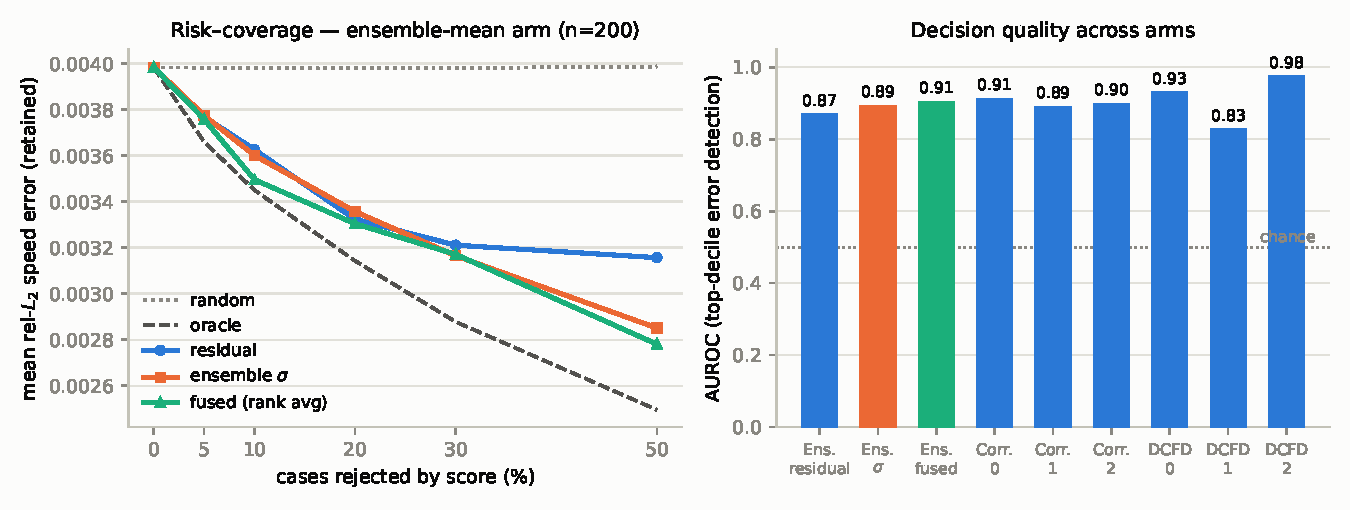
\includegraphics[width=0.95\textwidth]{../../results/figures/fig_risk_coverage.pdf}
\caption{\textbf{Selective prediction with the trust signal.} \emph{Left:} risk--coverage
curves on the AirfRANS test set (ensemble-mean arm): mean retained relative-$L_2$ error
after rejecting the least-trusted fraction of cases by physics residual, ensemble
$\sigma$, or their rank fusion, against the oracle (reject by true error) and random
rejection. \emph{Right:} AUROC for detecting worst-decile-error cases across arms
(AirfRANS ensemble-mean, three corrected seeds, three DeepCFD OOD seeds); chance $=0.5$.}
\label{fig:risk_coverage}
\end{figure}

\paragraph{On field error the physics does not earn its place; on drag it does.} A
\emph{physics-free} score---the ensemble $\sigma$, which needs no operator, no mesh and no
PDE---is nominally ahead of the residual ($0.894$ against $0.871$), and a paired
case-level bootstrap cannot separate them ($\Delta$AUROC $+0.023$, $95\%$ CI
$[-0.035,+0.083]$). The gain that survives is the \emph{fusion}'s. There is one place the
physics wins outright, and it is the place an engineer cares about: ranking cases by error
in the \emph{drag coefficient} rather than in the field, the residual reaches AUROC
$\mathbf{0.952}$, beating the physics-free score decisively ($\Delta$AUROC $+0.055$ to
$+0.088$, bootstrap CIs excluding zero).

\paragraph{The detector is not a difficulty proxy.} Cases whose geometry rasterises badly
could be both high-$\|r^\star\|$ and hard to predict, which would make the correlation a
restatement of case difficulty. Conditioning on each case's \emph{own} floor---the
ground-truth field's residual, an oracle quantity---leaves a partial rank correlation of
$0.561$ against a raw $0.610$, so $92\%$ of the association survives and the drop's CI
includes zero. The deployable residual also significantly outranks that oracle difficulty
variable itself, which a pure difficulty proxy could not do.

\paragraph{The acceptance gate is a throttle, not a filter---and what it buys is the
certificate.} Over $1200$ gated steps ($200$ AirfRANS \texttt{full} test cases $\times$ 3
seeds, on both the deployed Transolver$+$DEQ system and the ensemble-mean path, with the
accept rule, backtrack count and tolerance imported from the shipped
\texttt{correction\_loop}; \texttt{results/control/acceptance\_gate.json}), the test admits
a step on \textbf{$99.8\%$} of deployed cases---the \emph{full} correction on $50.7\%$ of
them---and refuses outright on one case in $600$. The mechanism is backtracking: where the
full step would raise the residual it is refused, but a halved step lowers it and is
admitted (on the ensemble path the residual ratio falls from a median $1.027$ at the full
step to $0.975$ at half). The admitted step lowers true rel-$L_2$ error on
\textbf{$89.3\%$} of deployed cases, by a median $\mathbf{5.8\%}$ ($74.3\%$ and $2.6\%$ on
the ensemble-mean path, where the correction has less headroom). But the obvious
control---an \emph{ungated} fixed half step, never consulting the residual---improves true
error on $95.8\%$ of deployed cases by a median $6.2\%$. \textbf{The gate's accuracy
advantage is therefore not there}; what improves the field is damping the correction, and
the residual test is not what earns that. What the gate uniquely buys is the
\textbf{certificate}: the ungated half step raises the monitored residual on $1.0\%$ of
deployed cases and $8.8\%$ on the ensemble path
(\texttt{results/review/control3\_fixed\_step.json}), and the gate makes that outcome
impossible by construction rather than improbable in practice. On the path a user actually
runs the guarantee binds on roughly one case in a hundred: it is a guarantee, not an
accuracy claim, and that is what we claim for it. (Scope: a single gated step applied
counterfactually to the deployed DEQ correction, which the shipped DEQ path bypasses by
design; not a re-run of the multi-iteration feed-forward loop of \autoref{tab:indist},
whose corrector checkpoints were not retained.)


% -----------------------------------------------------------------------------
% BLOCK 9 -- sec:cost, in full. Original body.tex lines 1656-1716, including
% tab:cost. The 1.13 ms audit cost and the 3822 ms deployed solve are quoted
% nowhere else once the trust layer is gone; their auditor rows were removed with
% this block.
% -----------------------------------------------------------------------------

\subsection{Computational cost}
\label{sec:cost}

A trust layer is only deployable if auditing costs materially less than the prediction it
audits. We time every stage of the deployed pipeline on the AirfRANS \texttt{full} test
set at resolution $128$ (\texttt{results/control/inference\_cost.json}; $100$ cases, median
of two timed repeats after an untimed warm-up, CUDA synchronised around each repeat, on
one RTX 4070 Ti with the package's single-thread BLAS cap in force).
\autoref{tab:cost} reports the result.

\begin{table}[t]
\centering
\small
\caption{\textbf{Per-case wall-clock cost of the deployed pipeline}
($128^2$ grid, $100$ AirfRANS \texttt{full} test cases, medians). \emph{Where} is the device
each stage actually runs on. The audit is the entire certificate: residual maps, trust map,
case-level score and conformal band. The classical anchor is the cost of generating one
AirfRANS case, as reported by its authors ($\approx 25$ min on $16$ CPU cores); it is
quoted for scale, not as a matched-hardware benchmark.}
\label{tab:cost}
\begin{adjustbox}{max width=\textwidth}
\begin{tabular}{l l r r l}
\toprule
stage & where & median & p95 & share of a deployed solve \\
\midrule
encode (geometry $\to$ input planes) & CPU, 1 thread & $1413$\,ms & $1620$\,ms & preprocessing \\
backbone forward + rasterise & GPU & $2080$\,ms & $3537$\,ms & $54.4\%$ \\
correction (Neural Residual Iteration) & GPU & $1747$\,ms & $2950$\,ms & $45.7\%$ \\
\midrule
\textbf{deployed solve} (backbone + correction) & GPU & $\mathbf{3822}$\,\textbf{ms} & $6400$\,ms & $100\%$ \\
\midrule
\textbf{audit} (residuals + trust + score + band) & CPU, 1 thread & $\mathbf{1.13}$\,\textbf{ms} & $2.49$\,ms & $\mathbf{0.03\%}$ \\
deep ensemble, $M{=}5$ (for the fused score) & GPU & $10\,114$\,ms & $10\,546$\,ms & $265\%$ \\
\midrule
classical steady-RANS solve \citep{bonnet2022airfrans} & 16 CPU cores & ${\sim}1\,500$\,s & --- & ${\sim}39\,000\%$ \\
\bottomrule
\end{tabular}
\end{adjustbox}
\end{table}

The audit costs $1.13$\,ms against a $3822$\,ms solve---one part in $3\,400$, or
$\mathbf{0.03\%}$; a conservative independent $200$-case re-measurement under CPU
contention gives $1.65$\,ms (\texttt{results/control/audit\_cost.json}). End to end a case
costs $5.24$\,s against the ${\sim}1500$\,s that produced its label. The deep-ensemble
spread does not share that property: measured by loading five independent backbones,
$M{=}5$ costs $4.86\times$ a single backbone---linear in $M$, confirmed rather than
assumed---which is $2.1$ deployed solves of \emph{extra} compute. This sharpens
\autoref{sec:selective} into a deployment choice: the residual alone recovers $\approx
67\%$ of the oracle's achievable error reduction at essentially zero marginal cost, while
fusing it with the ensemble spread reaches $\approx 91\%$ but triples the compute budget.
The audit's operation count is $O(N)$ in the number of grid cells; empirically, over a
$16\times$ range in $N$ ($64^2$ to $256^2$) it rises only $6.3\times$ (log--log slope
$0.64$, $R^2=0.99$), sub-linear because per-call fixed costs still dominate at these
sizes, so its share \emph{falls} as grids grow. These GPU figures are conservative upper
bounds rather than a tuned inference benchmark---the backbone stage times the Transolver
forward pass \emph{and} a single-threaded NumPy rasterisation, and the encode stage is
unoptimised preprocessing that any real design loop would cache. The classical anchor is
from the AirfRANS authors on $16$ CPU cores, so the ${\sim}286\times$ end-to-end figure
indicates the order of the gap, not a controlled speed-up. None of these caveats touches
the ratio the paper depends on---audit against solve---because both sides were measured in
the same run, on the same cases, under the same thread caps.


% -----------------------------------------------------------------------------
% BLOCK 10 -- "Reading against the pre-registered hypotheses", in full.
% Original body.tex lines 1805-1823. H1-H5 are all trust-layer or corrector
% hypotheses; the rebuilt manuscript's pre-registration is carried instead by
% rules D1-D3 (measure_asymmetry.py) and P1-P4 (point_space_headtohead.py),
% which are stated where they are read.
% -----------------------------------------------------------------------------

\subsection{Reading against the pre-registered hypotheses}

\textbf{H1 (the corrector improves accuracy):} \emph{backbone-dependent}---not supported
as pre-registered on the weak grid backbone, supported on the SOTA Transolver (all three
volume channels down on all 5 seeds, \autoref{tab:v2}). \textbf{H2 (the residual is a
valid trust signal):} \emph{supported, robustly}, in and out of distribution
($\rho>0$ for every arm/seed/split; DEQ lifts it to $0.83$ in-distribution and rescues the
\texttt{aoa} collapse $0.31\to0.75$), with two qualifiers stated in full in
\autoref{sec:selective}. \textbf{H3 (DEQ $\ge$ feed-forward corrector):} \emph{holds on the
design axis only}---DEQ wins on surface MSE, $\rho_{C_d}$ and the trust signal (3/3) and
loses on volume $\texttt{mse\_v}$/$\texttt{mse\_p}$. \textbf{H4 (conformal coverage):}
\emph{supported in-distribution}, \emph{empirical only} OOD; coverage was never in doubt,
width is what the floor costs. \textbf{H5 (DEQ contraction):} \emph{supported} (measured
factor $0.78 < \kappa = 0.9 < 1$). \textbf{Not pre-registered---the residual as a
correction \emph{objective}:} the registered set predates that experiment; we record for
completeness that had it been registered it would be \emph{falsified}
(\autoref{sec:residual}). Every number comes from the committed, reproducible harness
(\texttt{benchmarks/ablation.py}, \texttt{scripts/run\_certificates.py},
\texttt{results/sensitivity/}).


% -----------------------------------------------------------------------------
% BLOCK 11 -- the trust-layer limitations bullets. Original body.tex lines
% 1870-1878 (backbone-dependent correction), 1915-1926 (residual as objective vs
% the gate), 1927-1931 (two 2-D datasets), 1932-1947 (conformal coverage OOD and
% adaptivity), 1948-1950 (classical fallback stub).
% -----------------------------------------------------------------------------

\item \textbf{Backbone-dependent correction quality, and a third backbone that is not
like-for-like.} The supervised DEQ corrector reduces field MSE by $8$--$25\%$ on the SOTA
Transolver but is flat-to-unhelpful on the weak grid backbone; we report both and claim
only the latter. The trust signal is positive on all three backbones tested
($\rho=0.611$ Transolver, $\approx 0.40$--$0.83$ grid backbone, $0.851$ bare MeshGraphNet),
but the MeshGraphNet arm was trained on $16$k-point subsamples and evaluated at
$\approx180$k and our own density control returns \textsc{density-driven}, so the
matched-density range is $\rho\approx0.40$--$0.61$. We make no competitiveness claim for the
grid backbone; the Transolver backbone we run \emph{on} is itself competitive.

\item \textbf{The residual fails as an objective; the gate does not, and neither is the
source of the corrector's gain.} The DEQ contraction guarantee is in the correction
variable $\delta$, not in the output's PDE residual. The acceptance gate is a different
mechanism: measured, it admits a step on $99.8\%$ of deployed cases and that step lowers
true error on $89.3\%$ of them---though that measurement is a single gated step on the
deployed corrector, not the multi-iteration feed-forward loop, which remains untested at
this granularity, and an ungated half step does better on accuracy alone. Nor is the
$8$--$25\%$ field-MSE gain attributable to the residual as a corrector \emph{input}:
zeroing that input at train and inference (5 seeds) matches or slightly exceeds the
deployed corrector (WITH beats NULL on $0/5$ seeds), with one caveat stated in
\autoref{sec:method}---those channels are built from the wider differentiable stencil,
whose larger kernel we have not excluded.

\item \textbf{Two 2-D datasets; not yet 3-D.} The trust signal is validated on
turbulent-RANS AirfRANS airfoils and laminar DeepCFD bluff bodies ($\rho=0.77{\pm}0.12$),
so the phenomenon is not AirfRANS-specific, but all results remain 2-D. Extending the
residual verifier to 3-D \citep{ahmedml2024,elrefaie2024drivaernet} requires 3-D residual
operators and multi-TB, often unsteady datasets beyond a single-GPU budget.

\item \textbf{Conformal coverage out-of-distribution is empirical, not guaranteed, and
adaptivity needs an ensemble.} The distribution-free guarantee assumes exchangeability,
which fails under shift; OOD coverage holds in our experiments only because the uncertainty
inflates appropriately. Scores are pooled over spatially correlated cells, so the effective
sample size is below the raw cell count, and the calibration set is small ($n=100$). On the
near-deterministic Transolver, MC-dropout $\sigma$ is near-degenerate, so although coverage
holds ($0.902$) the quantile is $\approx 10^9$ and ECE $\approx 0.31$: coverage there is
delivered by a near-constant band. A deep ensemble of $M{=}5$ recovers an adaptive band
($q=2.35$, ECE $0.074$) at $5\times$ the training cost. Neither the split nor $M$ is the
remaining caveat---20 re-draws give coverage $0.899{\pm}0.009$, and sweeping every member
subset of size $M=2..5$ (26 subsets; \texttt{results/uq\_ensemble/mstudy.json}) leaves the
\emph{decision} layer insensitive (fused AUROC $0.905$--$0.912$, coverage $0.905$--$0.915$
at every $M$, so even $M{=}2$ supports triage) while band \emph{adaptivity} is what $M$
buys ($q$ inflates $2.35 \rightarrow 3.74 \rightarrow 9.98$ and ECE degrades $0.074
\rightarrow 0.113 \rightarrow 0.199$ as $M$ drops $5 \rightarrow 3 \rightarrow 2$, with
$M{=}4$ already close to $M{=}5$). Independently retrained ensembles remain future work.

\item \textbf{Classical fallback is a stub interface.} The trust-gated fallback fixes the
integration seam and reports what would run; the OpenFOAM/SU2 backends are not implemented
and bear on no quantitative claim.


% -----------------------------------------------------------------------------
% BLOCK 12 -- appendix figures that belonged to the cut sections.
% Original body.tex lines 2038-2057. fig:fig3 plotted the grid backbone's gap to
% Transolver and went with BLOCK 5; fig:cylinder went with BLOCK 6.
% -----------------------------------------------------------------------------

\begin{figure}[t]
\centering
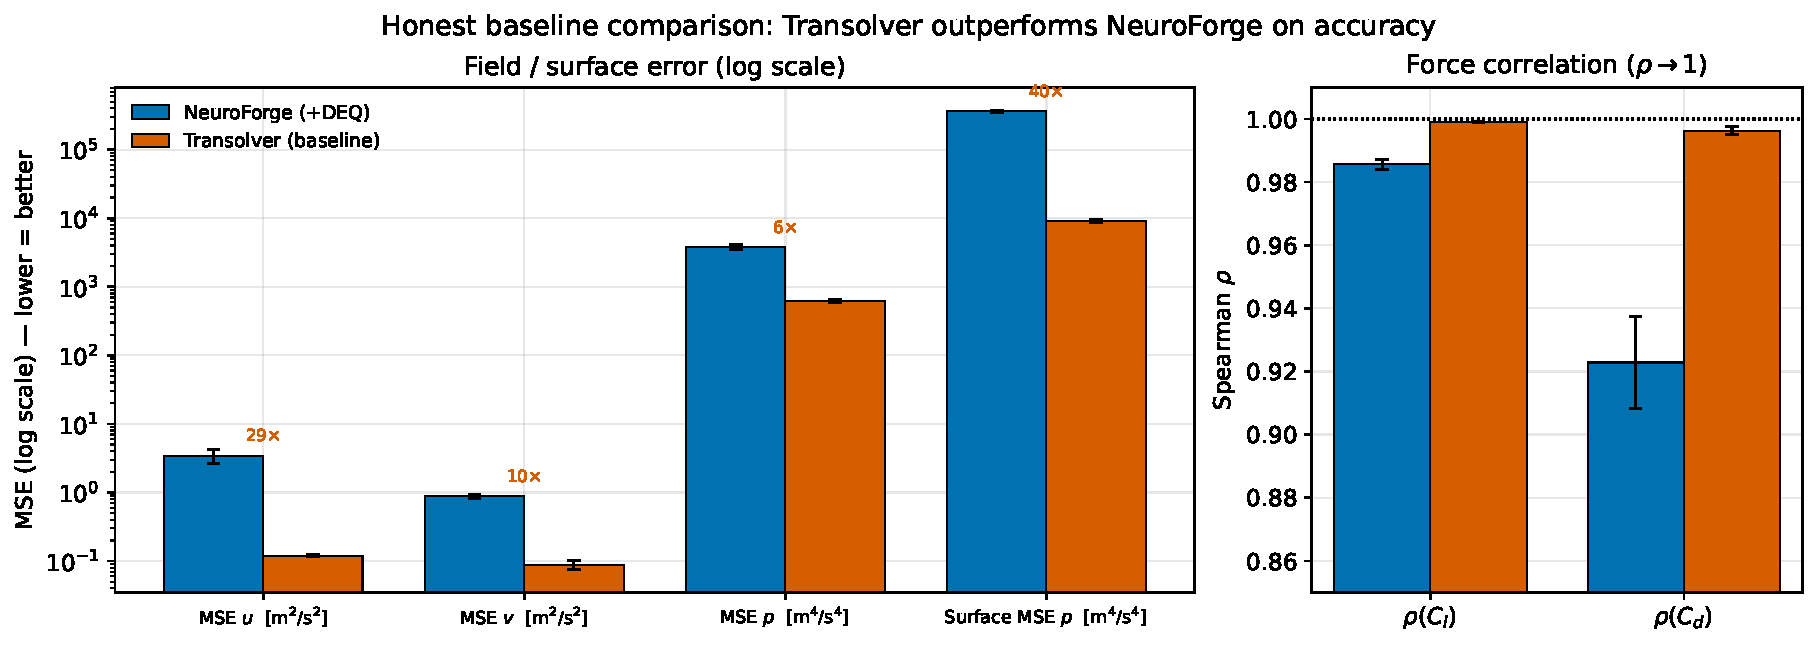
\includegraphics[width=0.85\textwidth]{../../results/figures/fig3_vs_transolver.pdf}
\caption{Matched-budget baseline (\autoref{tab:interp}): the grid backbone trails Transolver
$\sim 4$--$60\times$ across channels (no competitiveness claim).}
\label{fig:fig3}
\end{figure}

\begin{figure}[t]
\centering
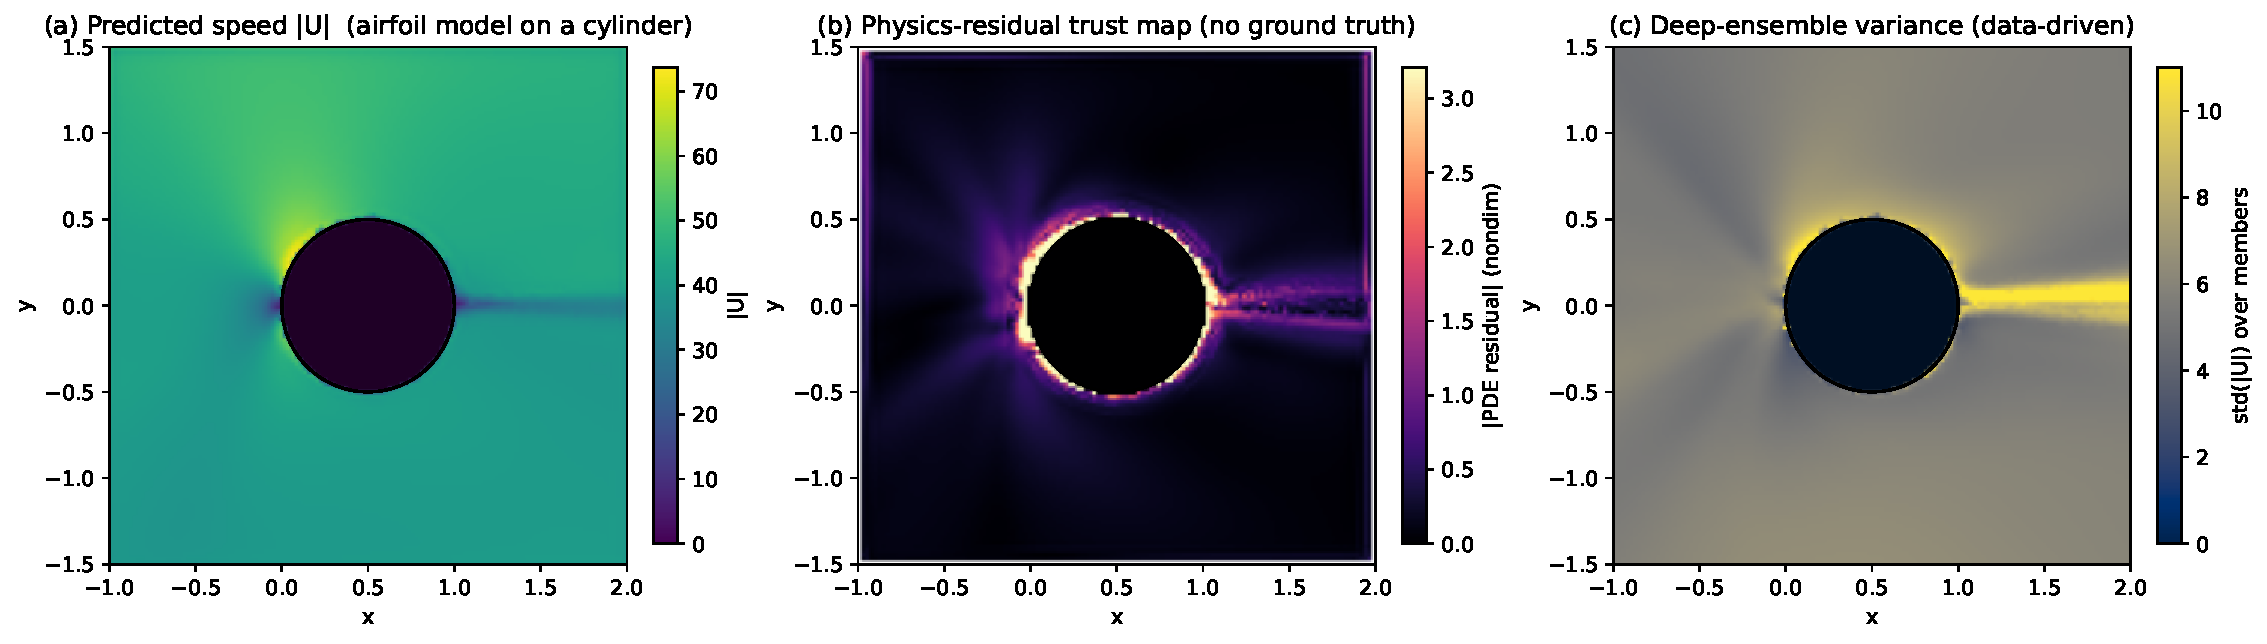
\includegraphics[width=\textwidth]{../../results/figures/fig_cylinder_ood.pdf}
\caption{Cross-geometry OOD (qualitative): an airfoil-trained model on a cylinder.
(a)~predicted speed (visibly broken); (b)~the physics-residual map (no ground truth used),
elevated field-wide; its bright near-body ring is a generic no-slip-wall feature common to
all bodies, \emph{not} an OOD localiser; (c)~deep-ensemble variance. The OOD signal is the
field-wide residual \emph{magnitude}---$\approx 7\times$ higher than in-distribution
airfoils in the far field, away from any wall (\autoref{sec:ood})---not its spatial
concentration.}
\label{fig:cylinder}
\end{figure}
